\documentclass{proc}
\bibliographystyle{ieeetr}

\usepackage{listings}
\usepackage{url}
\usepackage{multirow}
\usepackage{graphicx}

\lstset{
  basicstyle=\sffamily,
  columns=fullflexible,
  tabsize=2,
  frame=tb,
  captionpos=b,
}

\lstdefinelanguage{httpjson}{
  moredelim=[il][\bfseries]{~},
  literate={-}{-}{1}
}

\title{Newmograms: Authoring Interactive Nomograms for the Web}

\author{Claire Tuna \and Warren He}

\begin{document}

\maketitle

\begin{abstract}
We present a system that renders interactive nomograms on the web.
Our system is compatible with nomogram specifications designed for the
PyNomo package, modulo some minor encoding changes.
Our system uses PyNomo to precompute a dense sampling of points along
the nomogram's axes in order to suppor speedy interaction on
arbitrarily-shaped axes.
\end{abstract}

\section{Introduction}
Card and Mackinlay define nomograms as ``visual devices that allow
specialized computations''. Specifically, nomograms are analog
calculators through which a person can manipulate variables in
equations by drawing a line between two axes and reading the value off
of the third. They are traditionally hand-held devices, and before the
calculator, engineers used nomograms to aid with the graphical
calculations of multivariable formulas to a reasonable precision.

\section{Motivation}
The literature on nomograms suggests that though they are less
time-efficient than calculators, the user may develop some intuition
for the relationship between the variables in an equation. Cliff Stoll
in Scientific American writes that any engineer from the 1950s will
have ``a lament for the days when calculation went hand-in-hand with
deeper comprehension. Instead of plugging numbers into a computer
program, an engineer would understand the fine points of loads and
stresses, voltages and currents, angles and distances.''~\cite{sci-am}
We do not address the question of whether or not nomograms help aid
understanding, but we aim to bring the nomogram up to speed with the
digital calculator so that such a study may be possible in the future.

One issue with the physical nomogram that contributed to its fall from
grace was that ``slide rules had an Achilles' heel; standard models
could typically handle only three digits of precision.''~\cite{sci-am}
This lack of precision functions in many casual computations, but
could not compete with the calculator for tasks like “navigating the
path of a translunar space probe.''~\cite{sci-am} We address this
issue by leveraging the computers power to do fast calculations and
approximate to more decimals than the human can effectively read off
of a slide rule, for instance.

One route would be to develop a hybrid nomogram modeled after digital
calipers, with the precise, computer-generated output displayed on a
screen. This would provide the tactile interaction of the analog
nomogram with the advantages of precision. However, one use of
visualizations is to communicate information, and a nomogram on the
web is more portable and shareable than a physical nomogram. For this
reason, we implement a web based nomogram generating system.

\section{Related Work}

\subsection{PyNomo}
PyNomo~\cite{pynomo} is a nomogram authoring tool.
An author specifies a nomogram by choosing an equation template and
filling in mathematical functions and axis bounds.
The author can also specify numerical values to be drawn as lines.
PyNomo then generates a PDF of the nomogram.
Figure~\ref{fig:pynomo-pdf} shows an example of a nomogram generated
by PyNomo.
PyNomo runs as a Python package.

\begin{figure}
\label{fig:pynomo-pdf}
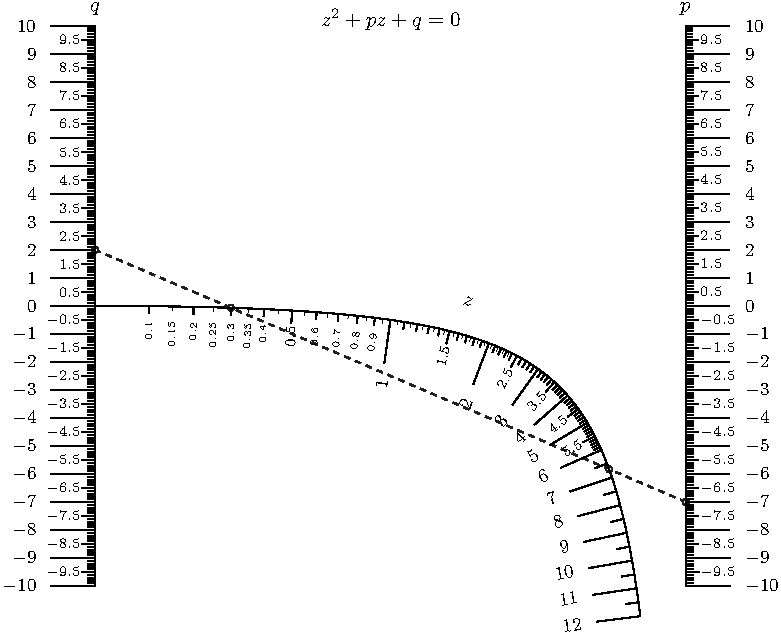
\includegraphics[width=\columnwidth]{ex_second_order_eq.pdf}
\caption{A nomogram generated by PyNomo.}
\end{figure}

We find that PyNomo is one of the most flexible nomogram authoring
tools available.
It supports a wide variety of equation types.
The ability to specify arbitrary functions to fill in the blanks in
its equation templates greatly increases its generality.
However, PyNomo only produces static nomograms.

\subsection{Interactive Nomogram Creation Tool}
Jones et al.'s Interactive Nomogram Creation Tool~\cite{jones-java} is
an interactive nomogram customization and presentation system.
This tool supports only the ``three-parallel-axes'' type of nomogram.
An author customizes the nomogram by changing the scales of the axes.
To interact with the nomogram, a user drags a line segment on the
screen, and the tool extends the line segment to intersect the axes.
Figure~\ref{fig:jones-java} shows a screenshot of the tool.

\begin{figure}
\label{fig:pynomo-pdf}
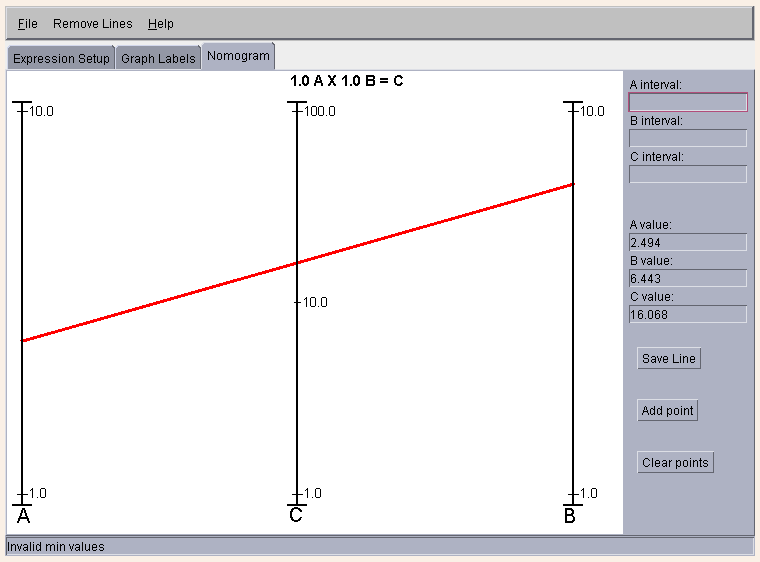
\includegraphics[width=\columnwidth]{jones-java.png}
\caption{A screenshot of Jones et al.'s Interactive Nomogram Creation
  Tool.}
\end{figure}

While Jones et al.'s tool provides an interactive visualization on the
web, it is limited in flexibility compared to PyNomo.
We find that the interaction drawing line segments interferes with an
advantage of nomograms, ``We could easily do `what if' calculations
just by adjusting slightly the position of the
ruler.''~\cite{card1999readings}
It is difficult to redraw the line segment to keep one axis point
fixed and adjusting another axis point slightly.

\section{Design Decisions}
\subsection{Fixed Axis Selection}
One important part of a linear nomogram is that 2 points determine the
line. When there are three axes, the user moves the pointer through
the values on the selected axis. In order to generate a line, one of
the other axes’ point position must remain fixed. In the physical
nomogram, if a user had a straight edge, they would hold down a point
with one hand and adjust the point on a second axis with the other
hand. In the WIMP model supported widely on desktop computers, there
is only one mouse.

We consider two different approaches for fixed axis selection:
automated and manual. In one approach, the fixed axis is automated
using a priority algorithm such as last recently used (LRU) remaining
fixed. When imagining the user’s interaction with the system, this
assumption that the LRU axis should remain fixed makes sense. A common
model in the equations represented by nomograms is that two of the
axes are inputs and the third is an output. In the BMI example, for
instance, if the user entered his/her weight and height and then
started adjusting the height, it seems natural that the weight should
remain fixed because the observed outcome is the BMI. However, the
automated approach introduces a modality which may hinder its
efficiency and also has decreased visibility and control by the user.
We could allow the user to click an axis to select it for staying
fixed and then move a point on a moveable axis. However, this approach
also introduces modality.

We propose a quasimode in which the user selects the fixed mode with
the left hand on the keyboard (keys 1, 2, 3 mapping to left, middle
and right) while selecting the moving axis with the mouse or trackpad.
This approach, like most translations, is a trade-off. The mapping
between the spacial relations of the axes in the nomogram and the
spatial relations between the 1-2-3 keys and the mouse hand are
imperfect. If the user is right handed, all of these keys are to the
left of the mouse, whereas the moving axis is not always the rightmost
one in the nomogram visualization. However, we hope that the key
selection (1-2-3), representing left most, middle, and right most,
presents a clear mental model to the user. We considered using a home
key such as F as an anchor (using S-D-F) as left-middle-right, and
this approach was tempting because the tactile memory would be greater
than keys with indistinguishable surfaces. However, we hope that the
user may be able to recognize 1-2-3 as the fixing-keys whereas the
motiviation for S-D-F is less clear on the surface.

The issue of handedness comes into play when designing such a
two-handed interface. The convention in computer games is to use the
arrow keys to designate left middle and right. However, this would not
suite a right-handed trackpad user, who would need to cross one arm
over the other to use the trackpad with the right hand and the arrow
keys with the left hand. For this reason, we keep one input tool
(1-2-3) far away from the other (the trackpad or mouse) to minimize
ergonomic awkwardness. If the user is left handed and using a
trackpad, their best solution would be to use the arrow keys as input.
Because it seems nearly impossible to optimize for both right and left
handed people, we accept both as input. This violates a design
guideline that there should be only one way to do a task and that way
should be the best way.~\cite{raskin} This guideline, however, is
motivated by the observation that when people alternate their input
method, they are slower to form habits. We do not anticipate this as
an issue because there will be different behavior between users (left
vs. right handed), but the vast majority of individual users, who
identify one dominant hand, would have no reason to switch back and
forth between the two. We predict that right handed users will
reliably use 1-2-3, whereas left handed users would use the arrow key.
We see no motivation for a right handed user to sometimes use the
arrows and sometimes use the numbers.

\section{Implementation}
We discuss the implementations of the two parts of our system: the
layout server and the renderer.

\subsection{Layout Server}
The layout server compiles a nomogram specification into an
intermediate format that contains precomputed points along each axis.
The server is a Flask~\cite{flask} application wrapped around a
modified version of PyNomo.

\subsubsection{Input}
Inputs to the server are almost the same format as for PyNomo.
PyNomo's specification format is a hierarchical arrangement of
key-value dictionaries.
An example is shown in Listing~\ref{lst:pynomospec}.
\lstinputlisting[language=Python,label=lst:pynomospec,caption={A
    PyNomo specification. This nomogram solves the equation
    $z^2+pz+q=0$}]{pynomo-spec.py}
Our server accepts a similar structure, but serialized as JSON.
The same example is shown in Listing~\ref{lst:ourspec}.
\lstinputlisting[language=httpjson,label=lst:ourspec,caption={An
    example request to our layout server, with a nomogram
    specification in JSON.}]{our-spec.json}

PyNomo allows an author to enter an arbitrary function as a lambda
function.
Our server also allows authors to specify their own functions, but
they must encode them as a JSON object with a \texttt{\_\_lambda\_\_} key
and the function body (in Python) as a string.
For security purposes, we place restrictions on what code we allow to
run.
Our server uses Python's parser to check the structure of the input
first.
Our lambda sanitization procedure only a few mathematically-useful
types of nodes to exist in the parse tree.
Table~\ref{tab:allowed-ast} lists these allowed node types.
\begin{table}
\label{tab:allowed-ast}
\begin{center}
\begin{tabular}{l|l}
\textbf{Node} & \textbf{Description} \\ \hline
BinOp & Binary operations, with... \\
Add & \multirow{5}{*}{Mathematical operators} \\
Sub \\
Mult \\
Div \\
Pow \\ \hline
Num & Numeric literals \\ \hline
Name & Names, which... \\
Load & Read a value
\end{tabular}
\end{center}
\caption{Our whitelist of parse tree nodes. User-provided lambda
  functions may contain only these nodes.}
\end{table}
We also allow names to occur, but we restrict them to a small list of
whitelisted functions from the standard \texttt{math} module.

The sanitizer also identifies up to one unbound variable for use as
the lambda's parameter name.
If the the parse tree satisfies these restrictions, the server
continues by finishing the compilation from this parse tree and
substituting the resulting \texttt{function} object into the
specification.

One additional nuance in converting from JSON to Python is that JSON
only supports one type of numeric data, while Python distinguishes
between floating point numbers and integers.
We parse all JSON numbers as floating point, so that PyNomo's internal
division operations continue to produce fractional results as
expected.

Finally, the server adds a few unchanging directives to the
specification: (1) a default paper size and (2) no output file.

At this point, the server has prepared an object that is a valid
PyNomo specification, with minimal formatting information.

\subsubsection{Customized PyNomo}
We run a modified version of PyNomo to compute a set of data for the
renderer to use.
A stock version of PyNomo lays out the nomogram's axes and renders
them to a PDF file at a specified path.
We have added additional code to PyNomo to expose the axis layout
information, which PyNomo normally discards after rendering the PDF.

We use the core \emph{logic} of PyNomo unmodified.
PyNomo lays out the axes as parametric curve for each variable.
This procedure for defining this curve based on the specification
depends on the nomogram type.
For each variable, PyNomo creates a function
$\Re\rightarrow\Re^2$ which map the value of the variable to a
coordinate.
(A catch-all ``general determinant'' nomogram type allows the author
to specify the parametric functions of these curves manually.)

PyNomo draws a parametric curve as a piecewise-linear appproximation.
It adaptively samples the curves' functions such that each line
segment is approximately a certain fraction of the curve's approximate
total length.
It also draws tickmarks by computing the curves' position and
derivative (finite difference numerical approximation) at round
numbers.
An author can configure PyNomo to prodcue up to five levels of tick
marks on each axis.

\subsubsection{Output}
Our server extracts the curve samples and tickmark positions and
orientation for each axis, in each nomogram.
The server returns this information in a JSON-serialized form.
Listing~\ref{lst:ourresponse} shows the structure of this response.
\lstinputlisting[language=httpjson,label=lst:ourresponse,caption={The
    structure of a response from our layout
    server.}]{our-response.json}

\subsection{Renderer}
A JavaScript application uses the D3.js library~\cite{d3js} to render
an interactive visualization based on the intermediate nomogram
representation compiled by the layout server.
This renderer uses the precomputed datapoints to guide the movement of
points.
Figure~\ref{fig:bmi-ours} shows a screenshot of an interactive
nomogram rendered by our system.

\begin{figure*}
\label{fig:bmi-ours}
\begin{center}
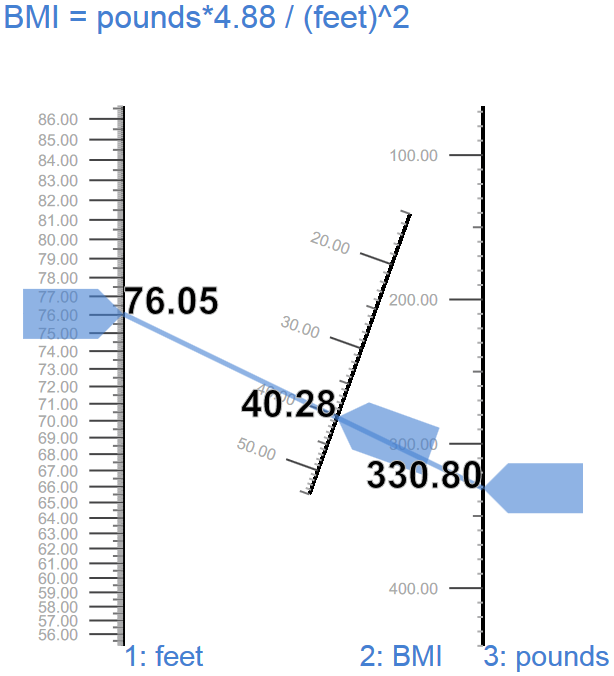
\includegraphics[width=0.9\textwidth]{bmi-ours.png}
\caption{A screenshot of an interactive nomogram rendered by our system.}
\end{center}
\end{figure*}

\subsubsection{Railed Draggable Handles}
In our design, the handles for moving the line shall stay on the axes.
While a user drags a handle, we position the handle at the closest
point on the axis associated with the dragged handle.
We search our precomputed point list of the axis for the point
physically closest to the cursor.

\subsubsection{Line Always Intersects Axes}
In our design, the line intersects every axis at least once.
To maintain this invariant, we prevent the line from moving into a
position such that it would no longer intersect with all the axes.
To implement this, we modify our algorithm for positioning the handle
during a dragging operation.
Instead of moving to the point closest to the cursor, the algorithm
only considers a point on the current axis if the line through that
point and the fixed point (on different axis) would pass through the
remaining axis.

We approximate the presence of an intersection by searching for the
point on the axis closest to the (infinite) line.
This algorithm considers the line to intersect the axis if the closest
point is within half a pixel of the line.
We found that the point sets from PyNomo are dense enough for this to
work.
An alternative algorithm is to check for intersections between the
(infinite) line and each line segment between consecutive points in
the axis's precomputed point list.

\subsubsection{Hiding the Slow Computations}
In one particular iteration of our renderer, the system would
explicitly check for both handle position and line position validity
continuously while the user dragged a handle.
This approach, which took a quadratic number of operations per
movement proved to be too slow.
To improve the smoothness of dragging, we instead compute line
position validity information in advance of any handle dragging
operation.
We precompute for each pair of axes $(fixed, moving)$, the validity of
each line through the current handle on $fixed$ and every point on
$moving$.
That is, if $check$ is the remaining axis, we compute, for every point
$p$ on $moving$, whether the line through the handle on $fixed$ and
$p$ intersects $check$.

Since these precomputed validity lookup structures are only valid for
a given configuration of the handles, we recompute this every time
\emph{after} the user drags any handle.
This way, our precomputation does not affect the smoothness during a
dragging operation.

\section{Results}
We discuss the performance aspects and limitations of our system.

\subsection{Layout Logic Platform}
We run PyNomo for its nomogram layout logic on a server.
This adds network delay to the nomogram authoring process.

Our modifications do not significantly affect PyNomo's performance.
We have only added operations to perserve the results of computations
that PyNomo would normally perform.
However, we do perform a few additional computations once PyNomo has
finished laying out the nomogram.
This primarily consists of additional evaluations of the axis
parametric functions in order to provide more data about the
tickmarks.

Overall, the added overhead of network delay and our additional
computation is small compared to the variance in PyNomo's execution
time running through the example nomograms from PyNomo's website.

\subsection{Discrete Sampled Axes}
Our use of precomputed points to represent an axis on the renderer
reduces our ability to provide high-precision results.
However, this allows us to achieve consistent performance regardless
of the complexity of parametric curves that define the axes.

\subsection{Handle Dragging Performance}
Although we do still loop through one axis to find the point closest
to the cursor, dragging a handle is smooth.
Our tests show that our visualization runs at full frame rate on a
modern MacBook Pro.

\subsection{Expensive Line Validity Computation}
Precomputing the line position validity information is the most costly
operation on the renderer.
The time it takes to do this operation increases quadratically with
the density of points on the axes and increases quadratically with the
number of axes in the nomogram.
This slow operation is noticeable in two cases: (1) opening the
nomogram and (2) releasing a handle and immediately dragging another.
Our tests show that this operation takes about one second for a
three-axis nomogram, each with around 1,000 points, on a modern
MacBook Pro.

\section{Discussion}

\subsection{The Cost of Generality}
The rationale for bearing these performance precision costs is to
support the generality offered by PyNomo.
While some forms of nomograms, such as those consisting of straight
lines, lend themselves to clean analytic solutions to the kind of
operations we need to perform, not all nomograms have such solutions.
It is not trivial to compute the intsersection of a line and a
general parametric curve.

\section{Future Work}
\subsection{Precise Input}
If the user wants to input a data point with many decimal places, they
will likely be dissatisfied with our system. In practice, it is hard
to move the slider to an exact value rather than an approximation.
This is one point that holds the nomogram back from competing with the
calculator. In a next iteration, the interactive nomogram could
include an input box for each axis such that the user could specify a
precise value if the dragging was too coarse. In the current
implementation, we only know a finite set of data points given to us
by PyNomo that the user can choose between. We interpret the drag as
corresponding to the nearest of these data points. Since there are
many points, usually the precision is fair. However, it fails to
encompass all combinations of numbers. The javascript has no knowledge
of the underlying function, and does not do calculations on the fly.
Perhaps in a future implementation, we can keep track of the exact
function so that we can do computations for novel data points inputted
by the user.

\subsection{A Touch Interface}
With the growing numbers of popular tablets and smartphones, we think
it would be useful to create a mobile, touch-based interface. We
designed the drag-points to be large and fingertip-sized with this
future in mind. Because a finger on the drag-points would result in
occlusion of any important text, we chose to put the numbers
indicating the values at the axes on top of the drag point, so the
value can be read off while the finger is in action. A touch interface
would also eliminate the need for the 1-2-3 quasimode, as the user
could touch two axes at once, no longer limited by the 1-handed mouse.
Because many nomograms are specific to the medical and construction
industries, it may also prove useful to have a mobile version to use
in the field. However, along with these advantages, we think that
touch would have its drawbacks. Precision may be difficult to achieve
to the exact decimal place that a person needs it if the only entry
method is through dragging. Additionally, three tick-dense axes may be
difficult to render legibly on, for example, an iPhone screen, which
is only 4.87 inches by 2.31 inches. With the 3 axes and two fingers on
the screen, it may be difficult to place everything such that nothing
important is occluded.

\subsection{Nomogram Annotation}
Many nomograms found online have one axis that is considered the
output of the other two. For example, in the BMI case, the inputs are
height and weight and the output is the BMI. In one BMI calculator
published on the website for the National Heart Lung and Blood
Institute, the calculator provides meaningful information about the
semantic meaning of the ranges of output, classifying them as
``Underweight'', ``Normal weight'', ``Overweight'' and ``Obesity''. If
the interactive nomogram hopes to replace such calculators, it should
also communicate the meaning of the calculation so that the user can
understand the results. We propose a future iteration in which after
the custom nomogram is generated, the user can modify it by adding
annotations to the output axis. In the case of the BMI, perhaps the
next iteration could have the range of the output (``Underweight'',
``Normal weight'', etc.) displayed live as well, or the axis could be
segmented into subsections of different colors. We leave this open for
discussion.

\bibliography{refs}

\end{document}
